\documentclass[a4paper, 10pt, twoside]{article}

\usepackage[top=1in, bottom=1in, left=1in, right=1in]{geometry}
\usepackage[utf8]{inputenc}
\usepackage[spanish, es-ucroman, es-noquoting]{babel}
\usepackage{setspace}
\usepackage{fancyhdr}
\usepackage{lastpage}
\usepackage{amsmath}
\usepackage{amsfonts}
\usepackage{amsthm}
\usepackage{verbatim}
\usepackage{graphicx}
\usepackage{float}
\usepackage{enumitem} % Provee macro \setlist
\usepackage{tabularx}
\usepackage{multirow}
\usepackage{hyperref}
\usepackage{multicol}
\usepackage[toc, page]{appendix}

\begin{document}


\tableofcontents

\newpage


\section{Introducción}

\section{Métodos y condiciones de cada experimento}
%Justificacion de la eleccion de S1
Para analizar la red se van a utilizar dos herramientas. Una que modela los paquetes Ethernet capturados como una fuente de información binaria de memoria nula $S$, definiendo el conjunto de símbolos que emite como ${S_{BROADCAST}, S_{UNICAST}}$. La segunda herramienta modela una fuente de información de memoria nula $S1$ que emite símbolos que son la IP destino de los paquetes $ARP$ de tipo $Who-has$ capturados. Un símbolo de esta fuente será distinguido cuando la información provista por el símbolo sea menor que la entropía de la fuente.

\subsection{Red de los labos}
Para este experimento se tomo una captura de 30 minutos de la red Wi-Fi de los labos de la facultad.

\section{Resultados}

\subsection{Red de los labos}

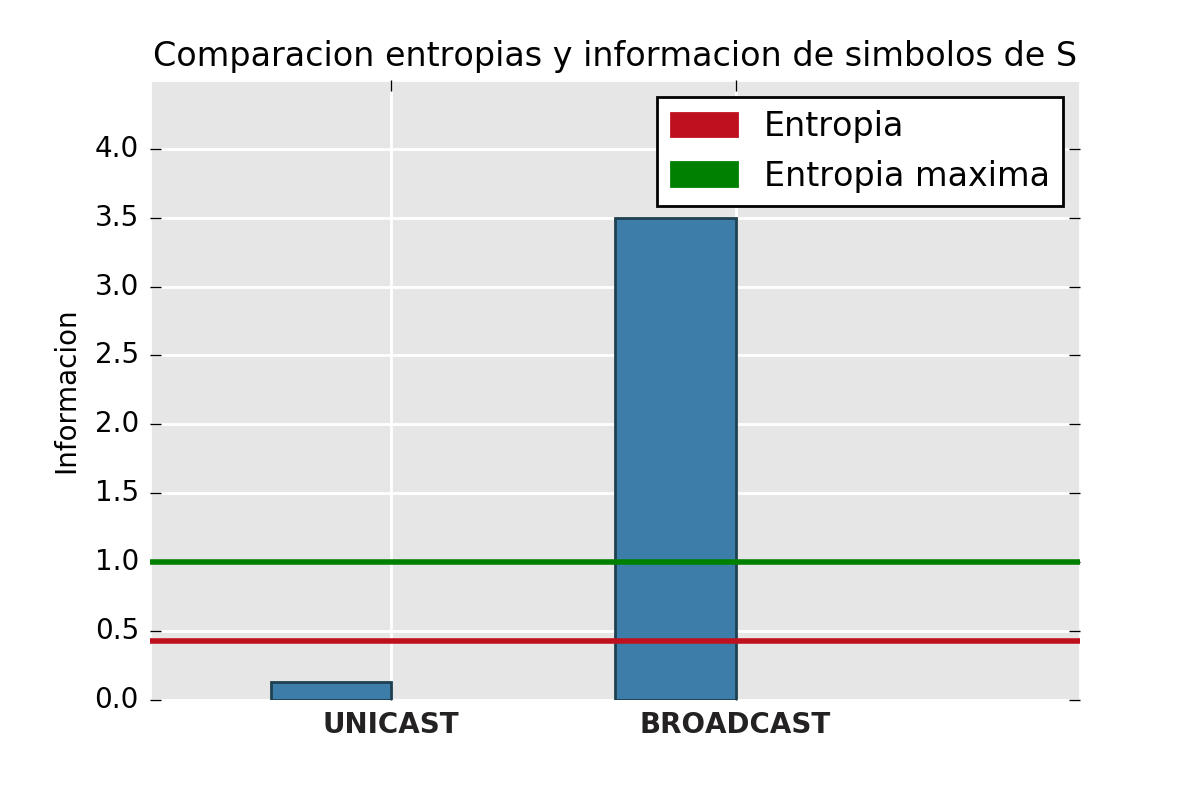
\includegraphics[height=10cm]{grafico1-red-labos.png} 

Como podemos ver en el gráfico comparativo la entropía no llega a ser máxima. De hecho puede verse en el símbolo BROADCAST proporciona mucha mas información que el símbolo UNICAST. Por lo que hay un mayor flujo de paquetes UNICAST que BROADCAST, "ACA UNA JUSTIFICACION SOBRE LO QUE SUGIERE ESTO ACERCA DE ESTA RED". 

El overhead impuesto por la red influencia la entropia de esta fuente. Por ejemplo, si hubiese mas mensajes $ARP$ $BROADCAST$ la información del símbolo $S_{BROADCAST}$ bajaría haciendo consecuentemente que la entropía de la fuente $S$ se vea modificada.

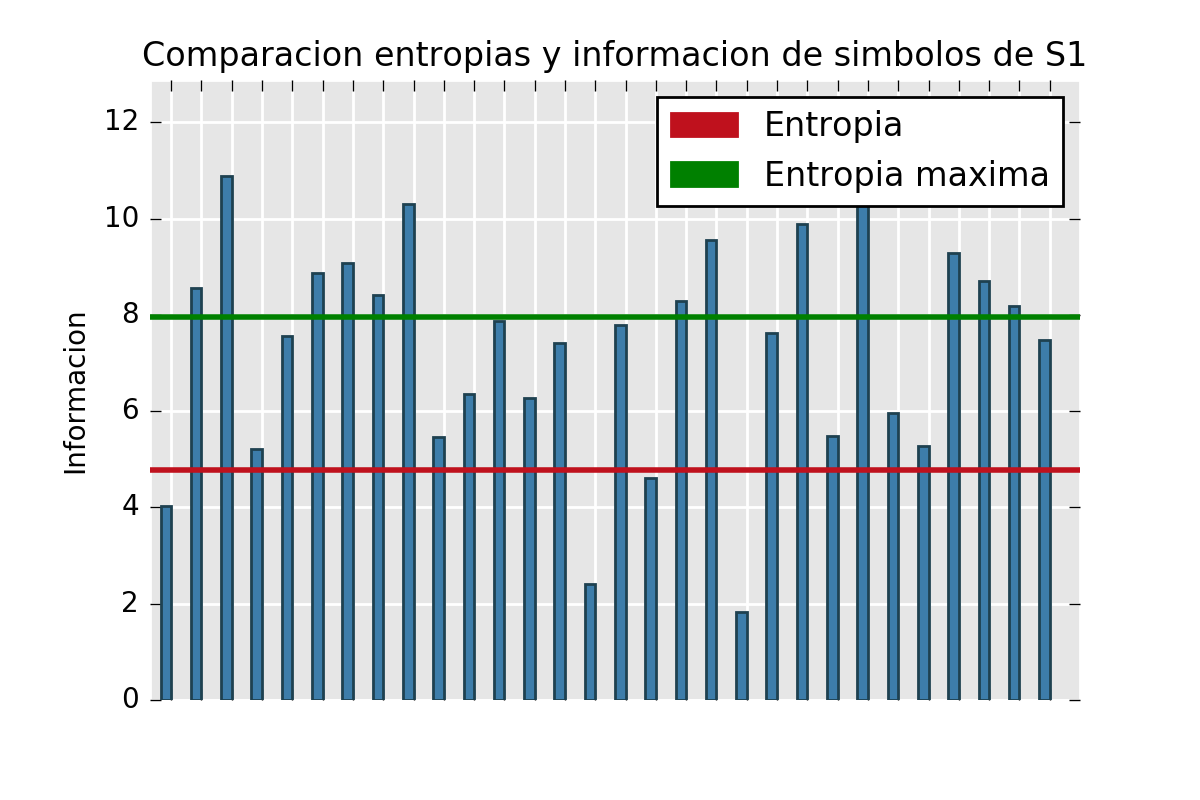
\includegraphics[height=10cm]{grafico2-red-labos.png} 

En comparación con el resto de los mensajes el tráfico $ARP$ es bajo, solo el 4\% de los mensajes son $ARP$. En base al criterio propuesto, se pueden distinguir 4 nodos:   

    \begin{table}[ht]\begin{center}
      \begin{tabular}{|c|c|}
      \hline
      \textbf{Nodo} & \textbf{Informacion} \\ \hline
      \texttt{10.2.7.254}& 1.829564 \\ \hline
      \texttt{10.2.203.254}& 2.414527 \\ \hline
      \texttt{10.2.1.250}& 4.026302 \\ \hline
      \texttt{10.2.3.254}& 4.601927 \\ \hline
      \end{tabular}
      \caption{Nodos destacados}
      \label{Nodos-destacados}
    \end{center}\end{table}

\section{Conclusión}


\end{document}
